\documentclass[11pt,letterpaper]{article}

% ------------------------------------------------------------
% CORE PACKAGES
% ------------------------------------------------------------
\usepackage[
  top=1in, bottom=1in, left=1in, right=1in,
  includeheadfoot
]{geometry}
\usepackage[T1]{fontenc}
\usepackage[utf8]{inputenc}
\usepackage{lmodern}
\usepackage{microtype}
\usepackage{amsmath,amssymb,mathtools}
\usepackage{xcolor}
\usepackage{tikz}
\usetikzlibrary{
  positioning, arrows.meta, quotes,
  calc, shapes.geometric, decorations.pathmorphing,
  decorations.markings, patterns, fadings
}
\usepackage{pgfplots}
\usepackage{pgfplotstable}
\pgfplotsset{compat=1.8}

\pgfplotsset{compat=newest}
\usepackage{tcolorbox}
\tcbuselibrary{skins,breakable,minted,theorems}
\usepackage{minted}
\usepackage{multicol}
\usepackage{booktabs}
\usepackage{array}
\usepackage{tabularx}
\usepackage{colortbl}
\usepackage{enumitem}
\usepackage{fancyhdr}
\usepackage{lastpage}
\usepackage{fontawesome5}
\usepackage{soul}
\usepackage{contour}
\usepackage{mdframed}
\usepackage{etoolbox}
\usepackage{fourier}
\usepackage{../Lectures/rahul_math}

% ------------------------------------------------------------
% METADATA (edit here)
% ------------------------------------------------------------
\newcommand{\course}{CPE 487/587}
\newcommand{\coursename}{Deep Learning for Engineering Applications}
\newcommand{\examnum}{Examination 1 Sample}
\newcommand{\semester}{Spring 2026}
\newcommand{\examdate}{February 26, 2026}
\newcommand{\examtime}{4:20 PM - 5:40 PM}
\newcommand{\instructor}{Dr. Rahul Bhadani}

% ------------------------------------------------------------
% COLOR PALETTE
% ------------------------------------------------------------
\definecolor{NavyDeep}{HTML}{A63D40}
\definecolor{NavyMid}{HTML}{1A3A5C}
\definecolor{NavyLight}{HTML}{2C527A}
\definecolor{GoldBright}{HTML}{F6AE2D}
\definecolor{GoldLight}{HTML}{0B1F3A}
\definecolor{GoldFill}{HTML}{FFFBEB}
\definecolor{CrimsonAccent}{HTML}{C1292E}
\definecolor{TealAccent}{HTML}{2E86AB}
\definecolor{TealLight}{HTML}{E0F4FA}
\definecolor{GreenAccent}{HTML}{235347}
\definecolor{MintFill}{HTML}{D8F3DC}
\definecolor{PurpleAccent}{HTML}{5C3784}
\definecolor{PurpleFill}{HTML}{F0EBF8}
\definecolor{SlateGray}{HTML}{64748B}
\definecolor{LightGray}{HTML}{F1F5F9}
\definecolor{MidGray}{HTML}{CBD5E1}
\definecolor{DarkGray}{HTML}{334155}
\definecolor{CodeBg}{HTML}{E0F4FA}
\definecolor{OffWhite}{HTML}{F8FAFC}
\definecolor{vggLightBlue}{RGB}{185, 220, 255}
\definecolor{vggDeepBlue}{RGB}{85, 180, 255}
\definecolor{blockblue}{RGB}{135,206,250}  % Light blue for main operations
\definecolor{blockwhite}{RGB}{255,255,255}  % White for 1x1 convs
\usepackage{graphicx} % Required for \resizebox

% Load TikZ libraries for positioning and arrows
\usetikzlibrary{positioning, arrows.meta}

% Define the custom colors used in your nodes and paths
\definecolor{GreenAccent}{RGB}{0, 150, 0}
\definecolor{NavyLight}{RGB}{100, 100, 255}
\definecolor{rnnCoral}{RGB}{255, 127, 80}

\usetikzlibrary{shapes.callouts}
\usetikzlibrary{arrows}
\usetikzlibrary{shapes.geometric, positioning}
\usetikzlibrary{matrix,positioning,decorations.pathreplacing,calc}

\usetikzlibrary{fit}
\tikzset{%
apple/.pic={
    \fill [MaterialBrown] (-1/8,0)  arc (180:120:1 and 3/2) coordinate [pos=3/5] (@)-- ++(1/6,-1/7)  arc (120:180:5/4 and 3/2) -- cycle;
    \fill [MaterialLightGreen500] (0,-9/10)  .. controls ++(180:1/8) and ++(  0:1/4) .. (-1/3,  -1) .. controls ++(180:1/3) and ++(270:1/2) .. (  -1,   0) .. controls ++( 90:1/3) and ++(180:1/3) .. (-1/2, 3/4) .. controls ++(  0:1/8) and ++(135:1/8) .. (   0, 4/7)
}
}
\usepackage{tikz-qtree,tikz-qtree-compat}
\usetikzlibrary{tikzmark}
\usetikzlibrary{calc}

\usetikzlibrary{positioning}

% ------------------------------------------------------------
% RANDOM DATA FOR PGFPLOTS
% ------------------------------------------------------------
\pgfmathsetseed{42}
\pgfplotstablenew[
  columns={z1,z2},
  create on use/z1/.style={create col/expr={rand}},
  create on use/z2/.style={create col/expr={rand}}
]{100}\dataplotOne
\pgfplotstablecreatecol[
  create col/expr={cos(30)*2.5*\thisrow{z1} - sin(30)*0.4*\thisrow{z2}}
]{x}{\dataplotOne}
\pgfplotstablecreatecol[
  create col/expr={sin(30)*2.5*\thisrow{z1} + cos(30)*0.4*\thisrow{z2}}
]{y}{\dataplotOne}

\pgfplotstablenew[
  columns={z1,z2},
  create on use/z1/.style={create col/expr={rand}},
  create on use/z2/.style={create col/expr={rand}}
]{100}\dataplotTwo
\pgfplotstablecreatecol[
  create col/expr={cos(120)*2.0*\thisrow{z1} - sin(120)*0.5*\thisrow{z2}}
]{x}{\dataplotTwo}
\pgfplotstablecreatecol[
  create col/expr={sin(120)*2.0*\thisrow{z1} + cos(120)*0.5*\thisrow{z2}}
]{y}{\dataplotTwo}

\pgfplotstablenew[
  columns={z1,z2},
  create on use/z1/.style={create col/expr={rand}},
  create on use/z2/.style={create col/expr={rand}}
]{100}\dataplotThree
\pgfplotstablecreatecol[
  create col/expr={cos(-45)*1.8*\thisrow{z1} - sin(-45)*1.2*\thisrow{z2}}
]{x}{\dataplotThree}
\pgfplotstablecreatecol[
  create col/expr={sin(-45)*1.8*\thisrow{z1} + cos(-45)*1.2*\thisrow{z2}}
]{y}{\dataplotThree}

% ------------------------------------------------------------
% TCOLORBOX STYLES
% ------------------------------------------------------------
\tcbset{
  % Section header
  sectionhead/.style={
    enhanced, arc=0pt,
    colback=NavyDeep, colframe=NavyDeep,
    colupper=white, fontupper=\bfseries\large,
    boxrule=0pt,
    left=12pt, right=12pt, top=7pt, bottom=7pt,
    overlay={
      \fill[GoldBright]
        ([xshift=0pt,yshift=0pt]frame.south west)
        rectangle
        ([xshift=4pt,yshift=0pt]frame.north west);
    },
    shadow={2pt}{-2pt}{0pt}{black!35},
  },
  % Warning / Instructions
  warning/.style={
    enhanced, breakable,
    colback=GoldFill, colframe=GoldBright,
    boxrule=1.5pt, arc=5pt,
    fonttitle=\bfseries\color{NavyDeep},
    colbacktitle=GoldBright,
    attach boxed title to top left={yshift=-2.5mm, xshift=8mm},
    boxed title style={arc=3pt, boxrule=0pt, colframe=GoldBright},
    left=10pt, right=10pt, top=12pt, bottom=8pt,
  },
  % Standard question box
  qbox/.style={
    enhanced, breakable,
    colback=OffWhite, colframe=TealAccent,
    boxrule=1.2pt, arc=4pt,
    left=9pt, right=9pt, top=7pt, bottom=7pt,
  },
  % Answer writing box
  abox/.style={
    enhanced, breakable,
    colback=white, colframe=GoldBright,
    boxrule=1.5pt, arc=5pt,
    fonttitle=\bfseries\small\color{white},
    colbacktitle=NavyMid,
    attach boxed title to top left={yshift=-2.5mm, xshift=8mm},
    boxed title style={arc=3pt, boxrule=0pt},
    left=9pt, right=9pt, top=14pt, bottom=8pt,
  },
  % True/False box
  tfbox/.style={
    enhanced, breakable,
    colback=white, colframe=GreenAccent,
    boxrule=1.2pt, arc=4pt,
    left=9pt, right=9pt, top=7pt, bottom=7pt,
  },
  % Multiple choice box
  mcbox/.style={
    enhanced, breakable,
    colback=white, colframe=TealAccent,
    boxrule=1.2pt, arc=4pt,
    left=9pt, right=9pt, top=7pt, bottom=7pt,
  },
  % Code box
  codebox/.style={
    enhanced, breakable,
    colback=white, colframe=PurpleAccent,
    boxrule=1.5pt, arc=5pt,
    fonttitle=\bfseries\small\color{white},
    colbacktitle=PurpleAccent,
    attach boxed title to top left={yshift=-2.5mm, xshift=8mm},
    boxed title style={arc=3pt, boxrule=0pt},
    left=9pt, right=9pt, top=14pt, bottom=8pt,
  },
  % Graph / data box
  graphbox/.style={
    enhanced, breakable,
    colback=white, colframe=GreenAccent,
    boxrule=1.5pt, arc=5pt,
    fonttitle=\bfseries\small\color{white},
    colbacktitle=GreenAccent,
    attach boxed title to top left={yshift=-2.5mm, xshift=8mm},
    boxed title style={arc=3pt, boxrule=0pt},
    left=9pt, right=9pt, top=14pt, bottom=8pt,
  },
  % Numeric answer cell
  numcell/.style={
    colback=white, colframe=GoldBright,
    boxrule=1pt, arc=3pt,
    left=4pt, right=4pt, top=3pt, bottom=3pt,
    halign=center, valign=center,
  },
  % Bonus box
  bonusbox/.style={
    enhanced,
    colback=white, colframe=PurpleAccent,
    boxrule=1.2pt, arc=5pt,
    fonttitle=\bfseries\small\color{white},
    colbacktitle=PurpleAccent,
    attach boxed title to top right={yshift=-2.5mm, xshift=-8mm},
    boxed title style={arc=3pt, boxrule=0pt},
    left=9pt, right=9pt, top=14pt, bottom=8pt,
  },
}

% ------------------------------------------------------------
% HELPER COMMANDS
% ------------------------------------------------------------
\newcommand{\pts}[1]{\hfill{\color{CrimsonAccent}\bfseries[#1 pts]}}
\newcommand{\numbox}[1][3.2cm]{%
  \begin{tcolorbox}[numcell,width=#1]\vspace{0.46cm}\end{tcolorbox}%
}
\newcommand{\blankS}{\underline{\hspace{3.0cm}}}
\newcommand{\blankM}{\underline{\hspace{5.5cm}}}
\newcommand{\blankL}{\underline{\hspace{8.5cm}}}

% Decorative section title command
\newcommand{\sectiontitle}[1]{%
  \begin{tcolorbox}[sectionhead]%
    #1%
  \end{tcolorbox}%
}

% TF answer pair
\newcommand{\TF}{\hfill%
  \tikz[baseline=-0.3ex]{
    \draw[NavyMid,thick] circle(1.1ex);
    \node[font=\bfseries\small,NavyMid] at (0,0) {T};
  }\hspace{6pt}%
  \tikz[baseline=-0.3ex]{
    \draw[NavyMid,thick] circle(1.1ex);
    \node[font=\bfseries\small,NavyMid] at (0,0) {F};
  }%
}

% ------------------------------------------------------------
% FANCYHDR (article class -- no conflict)
% ------------------------------------------------------------
\pagestyle{fancy}
\fancyhf{}
\setlength{\headheight}{34pt}
\renewcommand{\headrulewidth}{0pt}
\renewcommand{\footrulewidth}{0pt}

% Colored bar header via TikZ overlay
\fancyhead[L]{%
  \begin{tikzpicture}[remember picture, overlay]
    \fill[NavyDeep]
      (current page.north west)
      rectangle ([yshift=-1.15cm]current page.north east);
    \fill[GoldBright]
      ([yshift=-1.15cm]current page.north west)
      rectangle ([yshift=-1.33cm]current page.north east);
    % text lives INSIDE the tikzpicture, drawn after the fills
    \node[anchor=west, xshift=1cm, yshift=-0.57cm,
          text=white, font=\bfseries\normalsize]
      at (current page.north west) {\course\ --\ \coursename ~(UAH)};
    \node[anchor=east, xshift=-1cm, yshift=-0.57cm,
          text=white, font=\small\itshape]
      at (current page.north east) {\examnum\ \textbullet\ \semester};
  \end{tikzpicture}%
}
\fancyhead[R]{}


\fancyfoot[L]{%
  \begin{tikzpicture}[remember picture, overlay]
    % Gold accent stripe just above navy bar
    \fill[GoldBright]
      ([yshift=0.72cm]current page.south west)
      rectangle
      ([yshift=0.86cm]current page.south east);
    % Navy bar anchored to true bottom of page
    \fill[NavyDeep]
      (current page.south west)
      rectangle
      ([yshift=0.72cm]current page.south east);
    % Left: due date
    \node[anchor=west, xshift=1cm, yshift=0.36cm,
          text=white, font=\small]
      at (current page.south west) {\textbf{\examdate}};
    % Centre: colour squares
    \node[anchor=center, yshift=0.36cm]
      at (current page.south) {%
        \begin{tikzpicture}[baseline=-0.4ex]
          \foreach \i/\c in {0/TealAccent,0.55/GoldBright,1.1/NavyLight}{
            \fill[\c] (\i em,0) rectangle (\i em+0.45em, 0.25em);
          }
        \end{tikzpicture}};
    % Right: page number
    \node[anchor=east, xshift=-1cm, yshift=0.36cm,
          text=white, font=\small]
      at (current page.south east) {Instructor: \instructor ~~ | ~~ Page\ \thepage\ \textbf{/}\ \pageref{LastPage}};
  \end{tikzpicture}%
}
\fancyfoot[C]{}
\fancyfoot[R]{}

% First page has no running header -- we use a special style
\fancypagestyle{coverpage}{%
  \fancyhf{}%
  \renewcommand{\headrulewidth}{0pt}%
  \renewcommand{\footrulewidth}{0pt}%
}

\setlength{\parindent}{0pt}
\setlength{\parskip}{5pt}

\makeatletter
\renewcommand{\section}{%
  \@ifstar{\@sectionstar}{\@ifnextchar[{\@sectionopt}{\@sectionnoopt}}%
}

\def\@sectionstar#1{%
  \begin{tcolorbox}[sectionhead]%
    \enspace \textbf{--} #1%
  \end{tcolorbox}%
}

\def\@sectionopt[#1]#2{%
  \refstepcounter{section}%
  \addcontentsline{toc}{section}{#1}%
  \begin{tcolorbox}[sectionhead]%
    \enspace Section \thesection\ \textbf{--} #2%
  \end{tcolorbox}%
}

\def\@sectionnoopt#1{%
  \refstepcounter{section}%
  \addcontentsline{toc}{section}{#1}%
  \begin{tcolorbox}[sectionhead]%
    \enspace Section \thesection\ \textbf{--} #1%
  \end{tcolorbox}%
}
\makeatother


% ============================================================
\begin{document}
% ============================================================

% ============================================================
%  PAGE 1 -- COVER PAGE
% ============================================================
\thispagestyle{coverpage}

% ------------- Full-bleed decorative header (TikZ overlay) --
\begin{tikzpicture}[remember picture, overlay]

  % Deep navy background block
  \fill[NavyDeep]
    (current page.north west)
    rectangle
    ([yshift=-9.2cm]current page.north east);

  % Diagonal gold accent band
  \fill[GoldBright, opacity=0.92]
    ([yshift=-8.6cm]current page.north west)
    -- ([yshift=-8.6cm]current page.north east)
    -- ([yshift=-9.2cm]current page.north east)
    -- ([yshift=-8.8cm]current page.north west)
    -- cycle;

  % Thin teal stripe above gold
  \fill[TealAccent]
    ([yshift=-8.4cm]current page.north west)
    rectangle
    ([yshift=-8.6cm]current page.north east);

  % Subtle geometric circle decoration (top-right corner)
  \foreach \r in {1.8, 3.0, 4.2}{
    \draw[white, opacity=0.06, line width=1.4pt]
      ([xshift=-2.5cm, yshift=-4.5cm]current page.north east)
      circle (\r cm);
  }

  % Tiny dot-grid pattern (upper left area)
  \foreach \x in {1.2, 1.8, 2.4, 3.0, 3.6}{
    \foreach \y in {-1.0, -1.6, -2.2, -2.8, -3.4, -4.0, -4.6}{
      \fill[white, opacity=0.10]
        ([xshift=\x cm, yshift=\y cm]current page.north west)
        circle (1.1pt);
    }
  }

  % Large subtle "1" watermark
  \node[
    font=\fontsize{180}{180}\selectfont\bfseries,
    text=white, opacity=0.04,
    anchor=center,
  ] at ([xshift=0cm, yshift=-4.5cm]current page.north) {1};

  % Circuit-board style horizontal lines
  \foreach \y in {-5.8,-6.2,-6.6,-7.0}{
    \draw[TealAccent, opacity=0.18, line width=0.6pt]
      ([xshift=1.0cm, yshift=\y cm]current page.north west)
      -- ([xshift=5.5cm, yshift=\y cm]current page.north west);
  }
  \foreach \x in {1.5,2.5,3.5,4.5}{
    \fill[TealAccent, opacity=0.25]
      ([xshift=\x cm, yshift=-5.6cm]current page.north west)
      circle (2.2pt);
  }

  % Bottom page accent bar
  \fill[NavyDeep]
    (current page.south west)
    rectangle
    ([yshift=0.7cm]current page.south east);
  \fill[GoldBright]
    ([yshift=0.7cm]current page.south west)
    rectangle
    ([yshift=0.86cm]current page.south east);

\end{tikzpicture}

% ------------- Course badge (top-left of header) -----------
\begin{tikzpicture}[remember picture, overlay]
  \node[
    anchor=north west,
    xshift=1.1cm, yshift=-0.55cm,
    minimum width=2.2cm, minimum height=1.8cm,
    fill=GoldBright, rounded corners=5pt,
    inner sep=4pt, align=center,
  ] at (current page.north west) {%
    \color{NavyDeep}\bfseries\large\course
  };
\end{tikzpicture}

% ------------- Header text --------------------------------
\vspace{1.0cm}
\hspace{3.5cm}%
\begin{minipage}[t]{0.75\textwidth}
  \raggedright
  {\color{GoldBright}\fontsize{15}{12}\selectfont\bfseries\MakeUppercase{\semester}}\\[2pt]
  {\color{MidGray}\large Instructor:\ \instructor}
\end{minipage}

\vspace{0.70cm}

% ------------- Main title block ---------------------------
\begin{center}
  {\color{SlateGray}\fontsize{36}{42}\selectfont\bfseries\coursename}\\[6pt]
  \begin{tikzpicture}
    \fill[GoldBright] (0,0) rectangle (12cm, 0.12cm);
  \end{tikzpicture}\\[10pt]
  {\color{GoldLight}\fontsize{22}{26}\selectfont\bfseries\examnum}\\[4pt]
  {\color{PurpleAccent}\large\examdate\quad\textbullet\quad\examtime\quad\textbullet\quad100 Points}
\end{center}

% ------------- Neural network decoration (subtle) ----------
\begin{tikzpicture}[remember picture, overlay]
  % Small neural net icon on the right of header
  \begin{scope}[
    xshift=-1.5cm, yshift=-4.8cm,
    shift={(current page.north east)},
    every node/.style={circle, fill=white, opacity=0.18,
      minimum size=5pt, inner sep=0pt},
  ]
    % Input layer  (4 nodes: i1..i4)
    \node (ia) at (0, 0.00) {};
    \node (ib) at (0, 0.50) {};
    \node (ic) at (0, 1.00) {};
    \node (id) at (0, 1.50) {};
    % Hidden layer (3 nodes: h1..h3)
    \node (ha) at (0.6, 0.25) {};
    \node (hb) at (0.6, 0.75) {};
    \node (hc) at (0.6, 1.25) {};
    % Output layer (2 nodes: o1..o2)
    \node (oa) at (1.2, 0.50) {};
    \node (ob) at (1.2, 1.00) {};
    % Edges input->hidden
    \foreach \s in {ia,ib,ic,id}
      \foreach \d in {ha,hb,hc}
        \draw[white, opacity=0.12, line width=0.4pt] (\s) -- (\d);
    % Edges hidden->output
    \foreach \s in {ha,hb,hc}
      \foreach \d in {oa,ob}
        \draw[white, opacity=0.12, line width=0.4pt] (\s) -- (\d);
  \end{scope}
\end{tikzpicture}

\vspace{0.02cm}

% ------------- Instructions box ---------------------------
\begin{tcolorbox}[warning, title={\faExclamationTriangle\enspace Important Instructions}]
  \begin{multicols}{2}
    \begin{itemize}[leftmargin=0.4cm, itemsep=3pt, topsep=2pt]
      \item \textbf{Permitted:} One two-sided handwritten cheat sheets (letter size or smaller), calculator, pen/pencil, eraser
      \item \textbf{Prohibited:} textbooks, electronic devices, collaboration of any kind
      \item Read every question carefully; do not assume prior familiarity with phrasing
    \end{itemize}
    \columnbreak
    \begin{itemize}[leftmargin=0.4cm, itemsep=3pt, topsep=2pt]
      \item Use all provided space; request extra sheets if needed
      \item Write clearly -- illegible work receives \textbf{0 pts}
      \item \textbf{Circle} or \textbf{box} every final answer
      \item Show all work for partial credit on numerical sections
    \end{itemize}
  \end{multicols}
\end{tcolorbox}

\vspace{0.1cm}

% ------------- Student name box ---------------------------
\begin{tcolorbox}[
  enhanced,
  colback=OffWhite, colframe=NavyMid,
  boxrule=2pt, arc=7pt,
  shadow={3pt}{-3pt}{0pt}{black!20},
  left=14pt, right=14pt, top=10pt, bottom=10pt,
]
  \vspace{6pt}
  \begin{tabular*}{\linewidth}{@{}l@{\hspace{10pt}}l@{\hspace{30pt}}l@{\hspace{10pt}}l@{}}
    {\color{NavyMid}\bfseries Name:}
      & \underline{\hspace{6.8cm}}
    & {\color{NavyMid}\bfseries A\#:}
      & \underline{\hspace{3.5cm}} 
  \end{tabular*}
\end{tcolorbox}

\vspace{0.1cm}
\begin{center}
  \color{SlateGray}\small
  Total Pages:\ \textbf{\pageref{LastPage}}
  \quad\textbullet\quad
  \textit{By signing below you affirm adherence to the academic integrity policy.}
\end{center}
\begin{center}
  {\color{NavyMid}\bfseries Signature:}\quad\underline{\hspace{8cm}}
  
  \vspace{0.1cm}
  
{  \color{SlateGray}\small The University of Alabama in Huntsville (UAH)}
  
\end{center}

% ============================================================
%  PAGE 2 -- SCORE DISTRIBUTION
% ============================================================
\newpage

% Title
\begin{tcolorbox}[
  enhanced,
  colback=NavyDeep, colframe=NavyDeep,
  arc=0pt, boxrule=0pt,
  left=15pt, right=15pt, top=10pt, bottom=10pt,
  shadow={2pt}{-2pt}{0pt}{black!30},
]
  \begin{center}
    {\color{GoldBright}\bfseries\LARGE\faChartBar\enspace Score Distribution Sheet}\\[3pt]
    {\color{MidGray}\large\examnum\quad\textbullet\quad\course\ --\ \coursename\quad\textbullet\quad\examdate}
  \end{center}
\end{tcolorbox}

\vspace{14pt}

% ---------- Visual score table (TikZ) ----------------------
\begin{center}
\begin{tikzpicture}[
  box/.style={
    draw=NavyMid, fill=OffWhite, thick,
    minimum width=1.6cm, minimum height=1.4cm,
    rounded corners=2pt,
    font=\small,
  },
  labelbox/.style={
    fill=NavyDeep, text=white, draw=NavyDeep,
    minimum width=1.6cm, minimum height=0.7cm,
    rounded corners=2pt,
    font=\bfseries\large,
  },
  pointsbox/.style={
    fill=GoldBright, text=NavyDeep, draw=GoldBright,
    minimum width=1.6cm, minimum height=0.6cm,
    rounded corners=2pt,
    font=\bfseries\large,
  },
  scorebox/.style={
    fill=white, text=NavyDeep, draw=DarkGray,
    minimum width=1.6cm, minimum height=1.2cm,
    rounded corners=2pt,
    font=\large,
  },
]

% Column positions
\foreach \col/\qname/\pts in {%
  0/Q1/10,%
  1.8/Q2/10,%
  3.6/Q3/10,%
  5.4/Q4/5,%
  7.2/Q5/10,%
  9.0/Q6/15,%
  10.8/Q7/10,%
  12.6/Q8/10}{

  % Question label
  \node[labelbox] at (\col+0.8, 3.5) {\qname};

  % Max points badge
  \node[pointsbox] at (\col+0.8, 2.7) {\pts\ pts};

  % Score entry box
  \draw[DarkGray, thick, rounded corners=2pt]
    (\col, 0) rectangle (\col+1.6, 2.1);
  \node[font=\small\color{DarkGray}] at (\col+0.8, 1.9) {Score};
  \draw[MidGray, thin] (\col, 1.65) -- (\col+1.6, 1.65);
  
  

}

% Bonus column
\node[
  fill=PurpleAccent, text=white, draw=PurpleAccent,
  minimum width=1.6cm, minimum height=0.7cm,
  rounded corners=2pt, font=\bfseries\small,
] at (14.4+0.8, 3.5) {Bonus};

\node[
  fill=PurpleFill, text=PurpleAccent, draw=PurpleAccent,
  minimum width=1.6cm, minimum height=0.6cm,
  rounded corners=2pt, font=\bfseries\footnotesize,
] at (14.4+0.8, 2.7) {+15 pts};

\draw[PurpleAccent, thick, rounded corners=2pt]
  (14.4, 0) rectangle (14.4+1.6, 2.1);
\node[font=\small\color{PurpleAccent}] at (14.4+0.8, 1.9) {Score};
\draw[PurpleAccent!40, thin] (14.4, 1.65) -- (16.0, 1.65);

% Decorative separator
\draw[GoldBright, line width=1.5pt] (-0.1, -0.35) -- (16.1, -0.35);

% TOTAL box (centered below)
\node[
  fill=NavyDeep, text=GoldBright, draw=NavyDeep,
  minimum width=3.4cm, minimum height=0.8cm,
  rounded corners=3pt, font=\bfseries\normalsize,
] at (8.0, -0.95) {\faStar\enspace TOTAL SCORE};

\node[font=\large\bfseries\color{NavyDeep}, anchor=west] at (5.15, -2.5) {Raw Score};
\node[font=\large\color{SlateGray}, anchor=west]          at (5.15, -3.0) {out of 100};
\draw[GoldBright!60, thin] (8.2, -2.75) -- (10.8, -2.75);
% Row 2 -- Bonus
\node[font=\large\bfseries\color{NavyDeep}, anchor=west] at (5.15, -4.5) {+ Bonus};
\node[font=\large\color{SlateGray}, anchor=west]          at (5.15, -5.0) {optional};
\draw[GoldBright!60, thin] (8.2, -4.75) -- (10.8, -4.75);
% Row 3 -- Final
\node[font=\large\bfseries\color{NavyDeep}, anchor=west] at (5.15, -7.0) {Final Score};
\fill[GoldFill] (8.2, -6.0) rectangle (10.8, -8.0);
\draw[GoldBright, thin] (8.2, -6.0) rectangle (10.8, -8.0);

\end{tikzpicture}
\end{center}


% ============================================================
%  PAGE 3 -- SECTION 1: TRUE / FALSE  (25 pts)
% ============================================================
\newpage
\section{\faCheckSquare\enspace {--} True / False\hfill\textcolor{GoldBright}{10 Points}}

\vspace{4pt}
{\small\textit{For each statement, circle \textbf{T} (True) or \textbf{F} (False).
  Each question is worth \textbf{1 pts.} No partial credit.}}
\vspace{8pt}

\begin{tcolorbox}[tfbox]
  \begin{enumerate}[label=\textbf{\arabic*.}, leftmargin=*, itemsep=14pt]

    \item  The function 
\begin{align*}
g(z) = \begin{cases}
1, \quad z \geq \theta\\
0, \quad otherwise
\end{cases}
\end{align*}
is fully differentiable.
  \\  \TF 

    \item  Is it possible to implement a neural network in PyToch without inhering from \texttt{nn.Module}?
   \\ \TF

    \item The vanishing gradient problem becomes \emph{more} severe as network depth increases, particularly with saturating activations such as sigmoid and tanh.
  \\  \TF

    \item In a Convolutional Neural Network, filter weights are shared spatially across all locations of a given feature map.
\\    \TF

    \item The Adam optimizer maintains per-parameter adaptive learning rates by tracking exponentially decaying first and second moment estimates of the gradient.
 \\   \TF
    
    \item Predicting the glucose-level given patients helatmetric is a regression problem. \\ \TF
    
    \item I have got the training accuracy of 95\% while training a deep learning model for predicting WiFi strength given access point transmit power, antenna gain/direction, and WiFi channel/frequency. I should immediately declare victory and publish a paper based on the result. \\ \TF
    
    \item \texttt{uv venv -- python 3.12} creates a Python virtual environment with Python 3.12. \\ \TF


\item Coefficient of determination $R^2$ can also be applied to deep neural network based machine learning models. \\ \TF

\item Sigmoid function is not differentiable at least at one point. \\ \TF

  \end{enumerate}
\end{tcolorbox}

\newpage

% ============================================================
%  SECTION 2: MULTIPLE CHOICE  (15 pts)
% ============================================================
\section{\faListOl\enspace \textbf{--} Multiple Choice\hfill\textcolor{GoldBright}{10 Points}}

\vspace{4pt}
{\small\textit{Circle the single best answer. \textbf{1 pts each.} No partial credit.}}
\vspace{8pt}

\begin{tcolorbox}[mcbox]
  \begin{enumerate}[label=\textbf{Q\arabic*.}, leftmargin=*, itemsep=16pt]

    \item 
    
    
    Consider a Neural Network diagram:

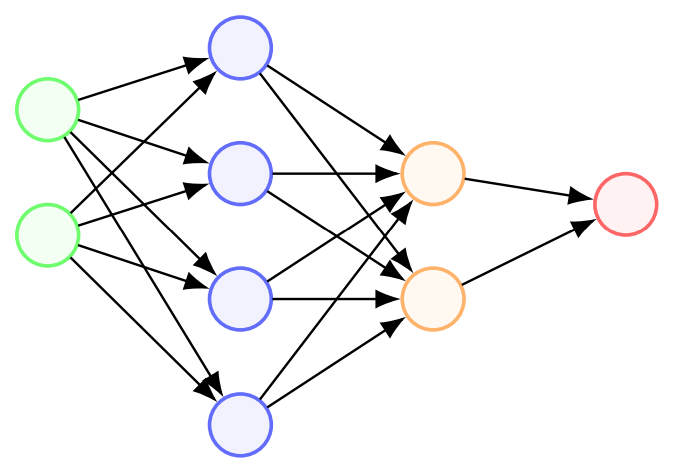
\includegraphics[width=0.5\linewidth]{../Classwork/figures/nn1.png}

If we are supplying two samples with two featurs (green bubbles), then what is the dimension of $W$s responsible for compressing 4 meta features to 2 meta features? For this assume that features in a feature matrix are along the column dimenions, and samples are along row dimensions.

    \begin{multicols}{4}
      \begin{enumerate}[label=(\Alph*), noitemsep]
\item $W_{4 \times 2}$
\item $W_{2 \times 4}$
\item $W_{4 \times 4}$
\item $W_{2 \times 2}$
      \end{enumerate}
    \end{multicols}


    \item A 2-D input of size $228 \times 228$ is passed through a convolutional layer with 64 filters of size $3\!\times\!3$, stride 1, and padding 1. What is the \textbf{spatial dimension} of the output feature map?
    \begin{multicols}{4}
      \begin{enumerate}[label=(\Alph*), noitemsep]
        \item $226 \times 226$
        \item $230 \times 230$
        \item $228 \times 228$
        \item $224 \times 224$
      \end{enumerate}
    \end{multicols}

    \item Consider a Network definition 

          \begin{minted}[
                linenos,
                frame=lines,
                framesep=2mm,
                bgcolor=pink!10,
                fontsize=\footnotesize,
                breaklines
            ]{Python}
class Network(nn.Module):
	def __init__(self):
		super().__init__()
		self.layer1 = nn.Linear(10, 20)
		self.layer2 = nn.Linear(20, 5)
	def forward(self, x):
		return self.layer2(self.layer1(x))
\end{minted}

How many trainable parameters are there in the above network (including biases)?

    \begin{multicols}{4}
      \begin{enumerate}[label=(\Alph*), noitemsep]
\item 325
\item 300
\item 55
\item 400
      \end{enumerate}
    \end{multicols}
    
    \item Which of the following is not an assumption in Simple Linear Regression model?
    
      \begin{enumerate}[label=(\Alph*), noitemsep]
\item 

\begin{align*}
\mathbb{E}[\epsilon_i] = 0 ~~ \forall ~~ i
\end{align*} 


\item 

\begin{align*}
\sigma^2[\epsilon_i] = \sigma^2 ~~ (\text{a constant}) ~~\forall i
\end{align*} 


\item 

\begin{align*}
\sigma[\epsilon_i, \epsilon_j] = 0 ~~  \forall ~~ i \neq j
\end{align*} 

\item 

\begin{align*}
\mathbb{E}[\epsilon_i^2] = 0 ~~ \forall ~~ i
\end{align*} 


      \end{enumerate}

\item Which of the loss function is not suitable for regression problems?

\begin{enumerate}
\item Cross-Entropy Loss
\item Mean-squared Error Loss
\item Mean absolute Error Loss
\item Total squared loss
\end{enumerate}

\item Consider an activation function as $\sigma(\xbf) = \frac{1}{1 + e^{-\xbf}}$ , if input is $\xbf = [1.09, 2.01, 3.0]$, the what is the dimension of $ A = \sigma(\xbf)$?

\begin{enumerate}

\item $3 \times 3$
\item $1$
\item Cannot be determined
\item $3$
\end{enumerate}

\item Consider a Neural Network definition:

          \begin{minted}[
                linenos,
                frame=lines,
                framesep=2mm,
                bgcolor=pink!10,
                fontsize=\footnotesize,
                breaklines
            ]{Python}
class QuizModel(nn.Module):
    def __init__(self):
        super().__init__()
        self.fc1 = nn.Linear(10, 5)
        self.relu = nn.ReLU()
        self.fc2 = nn.Linear(5, 2)

    def forward(self, x):
        x = self.fc1(x)
        x = self.relu(x)
        x = self.fc2(x)
        return x
\end{minted}

What is the size of the final output?

\begin{enumerate}
\item $2$
\item $5$
\item $1$
\item $2\times 5$
\end{enumerate}


\item Consider
\begin{align*}
\xbf = \begin{bmatrix}
1 \\ 2 \\ 4 \\ 6
\end{bmatrix}
\end{align*}
and 
\begin{align*}
\ybf = \fbf(\xbf) = \begin{bmatrix}
x_1 x_2 \\
x_1 + x_2\\
x_1x_2 + x_2x_3
\end{bmatrix}
\end{align*}

What is the size of Jacobian $J$?
\begin{enumerate}
\item  $4 \times 4$
\item $ 4\times 3$
\item $ 3\times 4$
\item $ 3 \times 3$
\end{enumerate}

\item Consider a convolution layer definition


          \begin{minted}[
                linenos,
                frame=lines,
                framesep=2mm,
                bgcolor=pink!10,
                fontsize=\footnotesize,
                breaklines
            ]{Python}
conv = nn.Conv2d(in_channels=4,  
                    out_channels=6, 
                    kernel_size=3, 
                    stride=2,
                    padding=1)
\end{minted}

What is the dimension of an example tensor that can serve as an input to the above convolution layer?

\begin{enumerate}
\item \texttt{torch.Size([2, 1, 5, 6])]}
\item \texttt{torch.Size([2, 6, 32, 32])]}
\item \texttt{torch.Size([2, 3, 5, 6])]}
\item \texttt{torch.Size([2, 4, 32, 32])]}
\end{enumerate}

\item Applying max pooling with a kernel size of $3\times 3$ to the image of size $5\times 5$ with a stride of $2$, the resulting output has size 

\begin{enumerate}
\item $2\times 2$
\item $3\times 3$
\item $5\times 5$
\item $3\times 5$
\end{enumerate}

  \end{enumerate}
\end{tcolorbox}

\newpage

% ============================================================
%  SECTION 3: SHORT ANSWER  (10 pts)
% ============================================================
\section{\faMarker\enspace \textbf{--} Short Answer\hfill\textcolor{GoldBright}{10 Points}}


{\small\textit{Answer each prompt in the box. Write in complete sentences. \textbf{5 pts each.}}}
\vspace{8pt}

\subsection{}
 Explain the intuition behind the \emph{attention mechanism} in transformers. Why is it more expressive than a fixed recurrent hidden state?
 \pts{5}
\vspace{5pt}
\begin{tcolorbox}[abox, title={Answer}, height=4.6cm, valign=top]
\vspace{1.5em}
\noindent\rule{\textwidth}{0.4pt}\\[1.5em]
\noindent\rule{\textwidth}{0.4pt}\\[1.5em]
\noindent\rule{\textwidth}{0.4pt}\\[1.5em]
\noindent\rule{\textwidth}{0.4pt}
\vspace{0.5em}
\end{tcolorbox}



\subsection{}

What happens if you don't register a member variable tensor as parameters in PyTorch \texttt{nn.Module}?
 \pts{5} 

\begin{tcolorbox}[abox, title={Answer}, height=4.6cm, valign=top]
\vspace{1.5em}
\noindent\rule{\textwidth}{0.4pt}\\[1.5em]
\noindent\rule{\textwidth}{0.4pt}\\[1.5em]
\noindent\rule{\textwidth}{0.4pt}\\[1.5em]
\noindent\rule{\textwidth}{0.4pt}
\vspace{0.5em}
\end{tcolorbox}


\subsection{}
Why does feedforward fully connected neural network not work well with sequential data? \pts{5} 



\begin{tcolorbox}[abox, title={Answer}, height=4.6cm, valign=top]
\vspace{1.5em}
\noindent\rule{\textwidth}{0.4pt}\\[1.5em]
\noindent\rule{\textwidth}{0.4pt}\\[1.5em]
\noindent\rule{\textwidth}{0.4pt}\\[1.5em]
\noindent\rule{\textwidth}{0.4pt}
\vspace{0.5em}
\end{tcolorbox}


\subsection{}
What is Markov assumption in n-Gram Language Model? \pts{5} 



\begin{tcolorbox}[abox, title={Answer}, height=4.6cm, valign=top]
\vspace{1.5em}
\noindent\rule{\textwidth}{0.4pt}\\[1.5em]
\noindent\rule{\textwidth}{0.4pt}\\[1.5em]
\noindent\rule{\textwidth}{0.4pt}\\[1.5em]
\noindent\rule{\textwidth}{0.4pt}
\vspace{0.5em}
\end{tcolorbox}


\newpage


\section{\faCalculator\enspace \textbf{--}  Mathematically Trained \hfill\textcolor{GoldBright}{10 Points}}

\subsection{}
An input feature matrix is 

\begin{align*}
I = \begin{bmatrix}
3 & 3 & 2 & 2 & 1 & 1\\
4 & 4 & 4 & 0 & 0 & 0\\
7 & 6 & 0 & 0 & 0 & 0\\
0 & 0 & 3 & 5 & 0 & 0
\end{bmatrix}
\end{align*}

Consider an averaging filter Kernel \begin{align*}
K = \frac{1}{9}\begin{bmatrix}
1 & 1  & 1\\
1 & 1  & 1\\
1 & 1  & 1\\
\end{bmatrix}
\end{align*}


 Consider a padding of 1 and stride of 1, and compute the output after applying the kernel to the input feature matrix.

\begin{tcolorbox}[qbox]

\bigskip

\bigskip

\bigskip

\bigskip

\bigskip

\bigskip

\bigskip

\bigskip

\bigskip

\bigskip

\bigskip

\bigskip

\bigskip

\bigskip

\bigskip

\bigskip

\bigskip


\end{tcolorbox}




\subsection{}


\newpage


\section{\faCalculator\enspace \textbf{--}  Forward Pass\hfill\textcolor{GoldBright}{5 Points}}

\vspace{4pt}
{\small\textit{Show all work for partial credit. Box or circle every final numeric answer.}}
\vspace{8pt}

\begin{tcolorbox}[qbox]
  \textbf{Problem 4.1} \pts{5}\quad Two-layer fully connected network:
  \begin{itemize}[noitemsep, leftmargin=*]
    \item Input: $\mathbf{x} = [1.0,\;0.5]^T$
    \item Layer 1:\; $W^{(1)} = \begin{bmatrix}0.2 & -0.3\\0.5 & 0.8\end{bmatrix}$,\;
      $\mathbf{b}^{(1)} = [0.1,\,-0.2]^T$,\; activation: \textbf{ReLU}
    \item Layer 2:\; $W^{(2)} = [0.6,\;-0.4]$,\;
      $b^{(2)} = 0.0$,\; activation: \textbf{Sigmoid}
  \end{itemize}

  \medskip
  \textbf{(a)} Compute $\mathbf{z}^{(1)} = W^{(1)}\mathbf{x} + \mathbf{b}^{(1)}$.\pts{1}

  \vspace{3.0cm}

  \textbf{(b)} Apply ReLU to obtain $\mathbf{a}^{(1)} = \text{ReLU}(\mathbf{z}^{(1)})$.\pts{1}

  \vspace{3.0cm}

  \textbf{(c)} Compute $\hat{y} = \sigma(W^{(2)}\mathbf{a}^{(1)} + b^{(2)})$.\pts{2}

  \vspace{3.0cm}

  \textbf{(d)} If $y = 1$, compute the binary cross-entropy loss.\pts{1}

  \vspace{3.0cm}

\end{tcolorbox}

\newpage

% ============================================================

\section{\faAtom\enspace \textbf{--} Magical CNN \hfill\textcolor{GoldBright}{10 Points}}

\vspace{4pt}

\begin{tcolorbox}[qbox]

  \medskip
  A CNN processes $3$-channel $224\!\times\!224$ images through:
  \begin{center}
  \renewcommand{\arraystretch}{1.35}
  \begin{tabular}{>{\bfseries}l c c c c}
    \toprule
    Layer   & Filters & Kernel         & Stride & Padding \\
    \midrule
    Conv1   & 32      & $3\!\times\!3$ & 1      & 1       \\
    Conv2   & 64      & $3\!\times\!3$ & 1      & 1       \\
    MaxPool & --      & $2\!\times\!2$ & 2      & 0       \\
    Conv3   & 128     & $3\!\times\!3$ & 1      & 1       \\
    \bottomrule
  \end{tabular}
  \end{center}
  
  
  \begin{enumerate}
  \item 
  \end{enumerate}

  \textbf{(a)} How many trainable are there parameters in \textbf{Conv1}?\pts{2}

  \vspace{3.0cm}

  \textbf{(b)} What is the spatial resolution after \textbf{MaxPool}?\pts{2}

  \vspace{3.0cm}

  \textbf{(c)} How many trainable parameters are there in \textbf{Conv3}?\pts{2}

  \vspace{3.0cm}
  
 

\end{tcolorbox}

\vspace{10pt}

%% ============================================================
%%  PAGE 5 -- SECTION 6: GRAPH INTERPRETATION  (15 pts)
%% ============================================================
%\newpage
%\sectiontitle{\faChartLine\enspace Section 6 \textbf{--} Graph Interpretation\hfill\textcolor{GoldBright}{15 Points}}
%
%\vspace{4pt}
%{\small\textit{Analyze the training curves and the PCA scatter plots below. Answer all sub-questions.}}
%\vspace{8pt}
%
%% Training curves
%\begin{tcolorbox}[graphbox, title={\faChartArea\enspace Figure 6.1 -- Training \& Validation Loss (Model A)}]
%  \begin{center}
%  \begin{tikzpicture}
%    \begin{axis}[
%      width=0.88\textwidth, height=5.8cm,
%      xlabel={\textbf{Epoch}},
%      ylabel={\textbf{Loss}},
%      xmin=0, xmax=50, ymin=0, ymax=2.5,
%      grid=both,
%      grid style={line width=0.3pt, draw=gray!20},
%      major grid style={line width=0.5pt, draw=gray!40},
%      tick label style={font=\small},
%      label style={font=\small\bfseries},
%      legend style={
%        at={(0.97,0.97)}, anchor=north east,
%        font=\small, fill=white, draw=MidGray,
%        rounded corners=2pt,
%      },
%      xtick={0,10,20,30,40,50},
%    ]
%      \addplot[color=TealAccent, ultra thick, smooth, domain=1:50, samples=60]
%        {0.15 + 1.8*exp(-0.12*x)};
%      \addlegendentry{Training Loss}
%
%      \addplot[color=CrimsonAccent, thick, dashed, domain=1:50, samples=60]
%        {0.40 + 1.6*exp(-0.10*x) + 0.013*(x-15)*max(0,x-15)/30};
%      \addlegendentry{Validation Loss}
%
%      \draw[GoldBright, thick, dashed] (axis cs:20,0) -- (axis cs:20,2.5);
%      \node[anchor=south, font=\tiny\bfseries, color=GoldBright]
%        at (axis cs:20,2.52) {Epoch 20};
%    \end{axis}
%  \end{tikzpicture}
%  \end{center}
%\end{tcolorbox}
%
%\vspace{8pt}
%
%% PCA scatter plots
%\begin{tcolorbox}[graphbox, title={\faSitemap\enspace Figure 6.2 -- PCA Scatter Plots (A, B, C)}]
%  \begin{center}
%  \begin{tikzpicture}
%    % Plot A
%    \begin{axis}[
%      name=plotA,
%      width=0.32\textwidth, height=4.2cm,
%      title={\small\textbf{(A)}},
%      xmin=-4,xmax=4, ymin=-4,ymax=4,
%      tick label style={font=\tiny},
%      grid=both, grid style={gray!15},
%      xlabel={\tiny $x_1$}, ylabel={\tiny $x_2$},
%    ]
%      \addplot[
%        only marks, mark=*, mark size=1.1pt,
%        color=TealAccent, opacity=0.7,
%      ] table[x=x,y=y]{\dataplotOne};
%    \end{axis}
%
%    % Plot B
%    \begin{axis}[
%      name=plotB,
%      at={(plotA.east)}, anchor=west, xshift=0.5cm,
%      width=0.32\textwidth, height=4.2cm,
%      title={\small\textbf{(B)}},
%      xmin=-4,xmax=4, ymin=-4,ymax=4,
%      tick label style={font=\tiny},
%      grid=both, grid style={gray!15},
%      xlabel={\tiny $x_1$}, ylabel={\tiny $x_2$},
%      yticklabels={},
%    ]
%      \addplot[
%        only marks, mark=*, mark size=1.1pt,
%        color=CrimsonAccent, opacity=0.7,
%      ] table[x=x,y=y]{\dataplotTwo};
%    \end{axis}
%
%    % Plot C
%    \begin{axis}[
%      name=plotC,
%      at={(plotB.east)}, anchor=west, xshift=0.5cm,
%      width=0.32\textwidth, height=4.2cm,
%      title={\small\textbf{(C)}},
%      xmin=-4,xmax=4, ymin=-4,ymax=4,
%      tick label style={font=\tiny},
%      grid=both, grid style={gray!15},
%      xlabel={\tiny $x_1$}, ylabel={\tiny $x_2$},
%      yticklabels={},
%    ]
%      \addplot[
%        only marks, mark=*, mark size=1.1pt,
%        color=GoldBright, opacity=0.7,
%      ] table[x=x,y=y]{\dataplotThree};
%    \end{axis}
%  \end{tikzpicture}
%  \end{center}
%\end{tcolorbox}
%
%\vspace{8pt}
%
%\begin{tcolorbox}[qbox]
%  \textbf{6.1}\pts{3}\enspace
%  Name the phenomenon visible in Figure 6.1 after Epoch 20. Explain what is happening to each curve.
%
%  \vspace{1.6cm}
%
%  \textbf{6.2}\pts{4}\enspace
%  List \textbf{three} techniques to mitigate the problem in 6.1. Briefly state the mechanism for each.
%
%  \vspace{2.5cm}
%
%  \textbf{6.3}\pts{4}\enspace
%  For Figure 6.2 scatter plots (A, B, C), estimate: (i) the direction of maximum variance for each, and (ii) which plot has the \emph{smallest} variance ratio between the two principal components.
%
%  \vspace{2.5cm}
%
%  \textbf{6.4}\pts{4}\enspace
%  In plot (A), if you project all points onto the first principal component, what fraction of the total variance is approximately \emph{retained}? Justify your estimate visually.
%
%  \vspace{2cm}
%\end{tcolorbox}

% ============================================================
%  PAGE 6 -- SECTION 7 & 8: CODING
% ============================================================
\newpage
\section{\faCode\enspace \textbf{--} Code Identification\hfill\textcolor{GoldBright}{10 Points}}

\vspace{6pt}

\begin{tcolorbox}[codebox, title={\faSearch\enspace Identify the Architecture (10 pts)}]

  \textit{Examine the PyTorch snippet below and answer the questions that follow.}

  \vspace{6pt}

\begin{minted}[
  bgcolor=CodeBg,
  fontsize=\small,
  linenos, numbersep=6pt,
  breaklines,
]{python}
import torch
import torch.nn as nn

class MysteryBlock(nn.Module):
    def __init__(self, in_channels, out_channels):
        super().__init__()
        self.branch1 = nn.Sequential(
            nn.Conv2d(in_channels, out_channels, kernel_size=1),
            nn.BatchNorm2d(out_channels),
            nn.ReLU(inplace=True),
            nn.Conv2d(out_channels, out_channels, kernel_size=3, padding=1),
            nn.BatchNorm2d(out_channels),
        )
        self.downsample = (
            nn.Conv2d(in_channels, out_channels, kernel_size=1)
            if in_channels != out_channels else nn.Identity()
        )
        self.relu = nn.ReLU(inplace=True)

    def forward(self, x):
        identity = self.downsample(x)
        out = self.branch1(x)
        out = out + identity          # <<< Line A
        return self.relu(out)
\end{minted}

\begin{enumerate}
\item What well-known deep learning architecture does \texttt{MysteryBlock} implement? \pts{2}
\item  What is the purpose of \textbf{Line A} and the \texttt{self.downsample} layer? Explain in 2--3 sentences.\pts{4}

\item  What specific training problem does this design help solve? Name the problem and state how this construction addresses it mathematically (hint: consider gradient flow).\pts{4}

\end{enumerate}
  
  


 

  \vspace{2.0cm}
\end{tcolorbox}


\newpage
\section{\faCode\enspace \textbf{--} Fancy Layers \hfill\textcolor{GoldBright}{10 Points}}


\subsection{}

Consider a VGG Block:

 \resizebox{0.3\textwidth}{!}{
            \begin{tikzpicture}[
                node distance=0.4cm,
                layer/.style={rectangle, draw=black, thick, minimum width=4.5cm, minimum height=0.6cm, font=\sffamily\small, align=center},
                conv/.style={layer, fill=vggLightBlue},
                pool/.style={layer, fill=vggDeepBlue},
                fc/.style={layer, fill=white},
                container/.style={rectangle, draw=black, thick, inner sep=0.3cm, rounded corners=2pt},
                arrow/.style={-Stealth, thick}
            ]

                % --- VGG BLOCK (LEFT) ---
                \node[conv] (b_c1) {$3 \times 3$ Conv, pad 1};
                \node[draw=none, above=0.3cm of b_c1] (b_dots) {\dots};
                \node[conv, above=0.3cm of b_dots] (b_c2) {$3 \times 3$ Conv, pad 1};
                \node[pool, above=0.3cm of b_c2] (b_p1) {$2 \times 2$ MaxPool, stride 2};
                
                % Container for VGG Block
                \node[container, fit=(b_c1) (b_p1), label={[font=\sffamily]above:VGG block}] (block_box) {};
                
                % Arrows for Block
                \draw[arrow] (b_c1) -- (b_dots);
                \draw[arrow] (b_dots) -- (b_c2);
                \draw[arrow] (b_c2) -- (b_p1);
                
                \end{tikzpicture}
                
          }
          

Provide an implementation for a composite layer \texttt{VGGBlock} representing above VGG Block implemented in PyTorch by inheriting from \texttt{nn.Module} class that specifies $v$ copies $3\times 3$ Conv Layer of padding 1 sequentially connected.

\begin{tcolorbox}[codebox]


\bigskip

\bigskip

\bigskip

\bigskip

\bigskip

\bigskip

\bigskip

\bigskip

\bigskip

\bigskip

\bigskip

\bigskip

\bigskip

\bigskip

\bigskip

\bigskip

\bigskip

\bigskip

\bigskip

\bigskip

\bigskip

\bigskip

\bigskip

\bigskip

\end{tcolorbox}

\subsection{}

Consider a quadratic equation $ h(\xbf) = a\xbf^2 + b \xbf + c$. Provide an implementation for a custom Neural Network Layer called QuadraticNet with $a, b,$ and $c$ as trainable parameters using PyTorch by inheriting from \texttt{nn.Module}.

\begin{tcolorbox}[codebox]


\bigskip

\bigskip

\bigskip

\bigskip

\bigskip

\bigskip

\bigskip

\bigskip

\bigskip

\bigskip

\bigskip

\bigskip

\bigskip

\bigskip

\bigskip

\bigskip

\bigskip

\bigskip

\bigskip

\bigskip

\bigskip

\bigskip

\bigskip

\bigskip

\bigskip

\bigskip

\bigskip

\bigskip

\bigskip

\bigskip

\bigskip

\bigskip

\bigskip

\bigskip

\bigskip

\bigskip

\bigskip

\bigskip

\bigskip

\end{tcolorbox}


\subsection{}


Consider a network shown below

 \resizebox{0.95\textwidth}{!}{
\begin{tikzpicture}[
                >=stealth, 
                node distance=1.8cm,
                neuron/.style={circle, draw=GreenAccent, fill=GreenAccent!20, thick, minimum size=1.2cm, font=\bfseries},
                input/.style={rectangle, draw=NavyLight, fill=NavyLight!20, thick, rounded corners=2pt, minimum size=1cm, font=\bfseries}
            ]
                % Nodes
                \node[input] (xt) {$x_t$};
                \node[neuron, right=of xt] (ht) {$h_t$};
                \node[neuron, right=of ht] (jt) {$j_t$};
                \node[neuron, right=of jt] (gt) {$g_t$};
                \node[neuron, right=of gt] (yt) {$y_t$};

                % Path connections
                \draw[->, thick] (xt) -- (ht);
                \draw[->, thick] (ht) -- (jt);
                \draw[->, thick] (jt) -- (gt);
                \draw[->, thick] (gt) -- (yt);
                
                % Recurrent Loop
                \draw[->, thick, rnnCoral] (ht.north) .. controls +(0.5,0.8) and +(-0.5,0.8) .. (ht.north) 
                    node[midway, above, font=\scriptsize] {$W_{hh}$};
                    
                 \draw[->, thick, rnnCoral] (gt.north) .. controls +(0.5,0.8) and +(-0.5,0.8) .. (jt.north) 
                    node[midway, above, font=\scriptsize] {$Q_{jg}$};
                
                % Label for context
                \node[below=0.3cm of ht, font=\scriptsize\itshape] {Hidden State 1};
                
                \node[below=0.3cm of gt, font=\scriptsize\itshape] {Hidden State 2};
            \end{tikzpicture}
}


Provide an implementation of above neural network with a recurrent connection and a feedback using PyTorch by inheriting from \texttt{nn.Module}. Assume that all nodes are performing linear affine transformation and in addition to recurrence and feedback they also apply linear affine transformation to regular inputs.

\begin{tcolorbox}[codebox]


\bigskip

\bigskip

\bigskip

\bigskip

\bigskip

\bigskip

\bigskip

\bigskip

\bigskip

\bigskip

\bigskip

\bigskip

\bigskip

\bigskip

\bigskip

\bigskip

\bigskip

\bigskip

\bigskip

\bigskip

\bigskip

\bigskip

\bigskip

\bigskip

\bigskip

\bigskip

\bigskip

\bigskip

\bigskip

\bigskip

\bigskip

\bigskip

\bigskip

\bigskip

\bigskip

\bigskip

\bigskip

\bigskip

\bigskip

\end{tcolorbox}



\newpage


\section{\faKeyboard\enspace \textbf{--} Sentence Probability\hfill\textcolor{GoldBright}{10 Points}}


Consider a text corpus


          \begin{minted}[
                linenos,
                frame=lines,
                framesep=2mm,
                bgcolor=pink!10,
                fontsize=\footnotesize,
                breaklines
            ]{html}
            
            <s> Washington had hoped to make a stand at New Brunswick, but was
disappointed</s>
            <s> New Brunswick is a province of Canada</s>
            <s> Washington has never been to Canada</s>
		 \end{minted}
	What is the probability of 
	
	\begin{minted}[
                linenos,
                frame=lines,
                framesep=2mm,
                bgcolor=pink!10,
                fontsize=\footnotesize,
                breaklines
            ]{html}
            <s>Washington had hoped to make a stand at Canada</s>
     \end{minted}
     
     using 2-gram model?

\begin{tcolorbox}[codebox]

\bigskip

\bigskip

\bigskip

\bigskip

\bigskip

\bigskip

\bigskip

\bigskip

\bigskip

\bigskip

\bigskip

\bigskip

\bigskip

\bigskip

\bigskip

\bigskip

\bigskip

\bigskip

\bigskip

\bigskip

\bigskip

\bigskip

\bigskip

\bigskip

\bigskip

\end{tcolorbox}



\newpage

\section{\faKeyboard\enspace \textbf{--} Embeddings\hfill\textcolor{GoldBright}{10 Points}}

Consider that after a particular epoch in the training embedding matrix looks like

\begin{align*}
E = \begin{bmatrix}
0.12 & 0.47 & 0.83 & 0.26 & 0.59 & 0.34 \\
0.71 & 0.05 & 0.62 & 0.48 & 0.91 & 0.17 \\
0.33 & 0.88 & 0.14 & 0.76 & 0.42 & 0.65 \\
0.56 & 0.29 & 0.73 & 0.08 & 0.84 & 0.51 \\
0.97 & 0.43 & 0.31 & 0.67 & 0.22 & 0.78 \\
0.15 & 0.64 & 0.52 & 0.39 & 0.86 & 0.03 \\
0.68 & 0.21 & 0.95 & 0.57 & 0.13 & 0.44 \\
0.82 & 0.36 & 0.07 & 0.93 & 0.61 & 0.28 \\
\end{bmatrix}
\end{align*}

Answer the following question

\begin{enumerate}
\item What is the $d_{model}$ of the embedding?
\item What is the size of vocabulary?
\item Write the one hot encoding matrix corresponding to the vocabulary.
\item Assuming that sequences ID assigned to tokens in the vocabulary start from 1, if a particular token sequence has been represented by $ T = \{4, 2, 1, 5, 3, 4 \}$, what is the emebdding for the given sequence?
\end{enumerate}

\begin{tcolorbox}[codebox]

\bigskip

\bigskip

\bigskip

\bigskip

\bigskip

\bigskip

\bigskip

\bigskip

\bigskip

\bigskip

\bigskip

\bigskip

\bigskip

\bigskip

\bigskip

\bigskip

\bigskip

\bigskip

\bigskip

\bigskip

\bigskip

\bigskip

\bigskip

\bigskip

\bigskip

\end{tcolorbox}


\newpage


% ============================================================

\section{\faKeyboard\enspace \textbf{--} Training Master \hfill\textcolor{GoldBright}{10 Points}}

\begin{enumerate}
\item 
\begin{tikzpicture}
\begin{axis}[
    width=12cm,
    height=8cm,
    xlabel={\large Epochs},
    ylabel={\large Loss},
    xlabel style={font=\large, below=2mm},
    ylabel style={font=\large, left=2mm},
    xmin=0, xmax=55,
    ymin=0.05, ymax=1.05,
    xtick={0,5,10,15,20,25,30,35,40,45,50},
    ytick={0.1,0.2,0.3,0.4,0.5,0.6,0.7,0.8,0.9,1.0},
    legend pos=north east,
    legend style={font=\normalsize, draw=black, fill=white, rounded corners=2pt},
    grid=both,
    grid style={line width=0.3pt, draw=gray!30},
    major grid style={line width=0.5pt, draw=gray!60},
    tick label style={font=\normalsize},
    title={\large Training vs.\ Validation Loss},
    title style={yshift=2mm},
    axis line style={thick},
]

%% --- Training Loss: consistently decreasing ---
\addplot[
    color=blue!80!black,
    line width=2pt,
    mark=*,
    mark size=1.8pt,
    mark options={fill=blue!80!black},
] coordinates {
    (1,  0.95)
    (2,  0.88)
    (3,  0.81)
    (4,  0.75)
    (5,  0.69)
    (6,  0.64)
    (7,  0.59)
    (8,  0.54)
    (9,  0.50)
    (10, 0.46)
    (11, 0.43)
    (12, 0.40)
    (13, 0.37)
    (14, 0.34)
    (15, 0.32)
    (16, 0.30)
    (17, 0.28)
    (18, 0.26)
    (19, 0.245)
    (20, 0.23)
    (21, 0.215)
    (22, 0.20)
    (23, 0.19)
    (24, 0.18)
    (25, 0.17)
    (26, 0.16)
    (27, 0.152)
    (28, 0.145)
    (29, 0.138)
    (30, 0.132)
    (31, 0.126)
    (32, 0.120)
    (33, 0.115)
    (34, 0.110)
    (35, 0.106)
    (36, 0.102)
    (37, 0.098)
    (38, 0.095)
    (39, 0.092)
    (40, 0.089)
    (41, 0.086)
    (42, 0.084)
    (43, 0.082)
    (44, 0.080)
    (45, 0.078)
    (46, 0.076)
    (47, 0.074)
    (48, 0.072)
    (49, 0.071)
    (50, 0.070)
};
\addlegendentry{Training Loss}

%% --- Validation Loss: decreases then increases ---
\addplot[
    color=red!80!black,
    line width=2pt,
    mark=square*,
    mark size=1.8pt,
    mark options={fill=red!80!black},
    dashed,
] coordinates {
    (1,  0.97)
    (2,  0.90)
    (3,  0.83)
    (4,  0.77)
    (5,  0.71)
    (6,  0.66)
    (7,  0.61)
    (8,  0.57)
    (9,  0.53)
    (10, 0.49)
    (11, 0.46)
    (12, 0.44)
    (13, 0.42)
    (14, 0.40)
    (15, 0.385)
    (16, 0.372)
    (17, 0.362)
    (18, 0.355)
    (19, 0.350)
    (20, 0.348)
    (21, 0.347)  %% << minimum ~ epoch 21
    (22, 0.350)
    (23, 0.355)
    (24, 0.362)
    (25, 0.372)
    (26, 0.385)
    (27, 0.400)
    (28, 0.418)
    (29, 0.438)
    (30, 0.460)
    (31, 0.484)
    (32, 0.510)
    (33, 0.536)
    (34, 0.562)
    (35, 0.588)
    (36, 0.613)
    (37, 0.637)
    (38, 0.660)
    (39, 0.682)
    (40, 0.703)
    (41, 0.722)
    (42, 0.740)
    (43, 0.757)
    (44, 0.773)
    (45, 0.788)
    (46, 0.802)
    (47, 0.815)
    (48, 0.827)
    (49, 0.838)
    (50, 0.848)
};
\addlegendentry{Validation Loss}



\end{axis}
\end{tikzpicture}

By looking at the above graph, when would have been the best time to stop training the neural network??

\item 

\textbf{Activation Functions}


\textit{Identify the different activation functions.}

 \textit{Which curve suffers from saturation or dying neurons?}

\begin{tikzpicture}
\begin{axis}[
    width=14cm,
    height=9cm,
    xlabel={\large Input $z$},
    ylabel={\large Output $f(z)$},
    xlabel style={font=\large},
    ylabel style={font=\large},
    xmin=-8, xmax=8,
    ymin=-1.6, ymax=1.6,
    xtick={-10, -9, -8, -7, -6,-5,-4,-3-2,-10,1,2,3,4,5,6,7,8,9,10},
    ytick={-1.5,-1,-0.5,0,0.5,1,1.5},
    legend pos=south east,
    legend style={
        font=\normalsize,
        draw=black,
        fill=white,
        rounded corners=3pt,
        row sep=2pt,
    },
    grid=both,
    grid style={line width=0.3pt, draw=gray!25},
    major grid style={line width=0.6pt, draw=gray!55},
    tick label style={font=\normalsize},
    title style={font=\Large, yshift=3mm},
    axis line style={thick},
    axis lines=center,      % puts axes through origin
    axis line style={-stealth, thick},
    clip=true,
]

%% ---- (A) Sigmoid: 1/(1+exp(-x)) -------------------------
\addplot[
    domain=-6:6, samples=300,
    color=blue!80!black, line width=2.2pt,
] { 1 / (1 + exp(-x)) };
\addlegendentry{$\mathbf{A}$}

%% ---- (B) Tanh ------------------------------------------
\addplot[
    domain=-6:6, samples=300,
    color=red!75!black, line width=2.2pt, dashed,
] { tanh(x) };
\addlegendentry{$\mathbf{B}$}

%% ---- (C) ReLU: max(0,x) --------------------------------
\addplot[
    domain=-6:6, samples=300,
    color=orange!90!black, line width=2.2pt, dotted,
] { max(0,x) };
\addlegendentry{$\mathbf{C}$}




\end{axis}
\end{tikzpicture}


\item 

\textbf{Derivatives of Activation Functions} 


\textit{Identify differenti activation functions based on their derivatives.}

\textit{Where does the gradient vanish or die?}

% ===========================================================
%  FIGURE 2 — Gradient / derivative plot
% ===========================================================
\begin{tikzpicture}
\begin{axis}[
    width=14cm,
    height=7cm,
    xlabel={\large Input $z$},
    ylabel={\large $f'(z)$ (Gradient)},
    xlabel style={font=\large},
    ylabel style={font=\large},
    xmin=-10, xmax=10,
    ymin=-0.2, ymax=1.35,
    xtick={-10, -9, -8, -7, -6,-5,-4,-3-2,-10,1,2,3,4,5,6,7,8,9,10},
    ytick={0,0.25,0.5,0.75,1.0,1.25},
    legend pos=north west,
    legend style={
        font=\normalsize,
        draw=black, fill=white,
        rounded corners=3pt,
        row sep=2pt,
    },
    grid=both,
    grid style={line width=0.3pt, draw=gray!25},
    major grid style={line width=0.6pt, draw=gray!55},
    tick label style={font=\normalsize},
    title style={font=\large, yshift=3mm},
    axis line style={thick},
    axis lines=center,
    axis line style={-stealth, thick},
    clip=true,
]

%% ---- (A) Sigmoid derivative: sigma*(1-sigma) ------------
\addplot[
    domain=-6:6, samples=300,
    color=blue!80!black, line width=2.2pt,
] { (1/(1+exp(-x))) * (1 - 1/(1+exp(-x))) };
\addlegendentry{$\mathbf{A}$}

%% ---- (B) Tanh derivative: 1 - tanh^2 -------------------
\addplot[
    domain=-6:6, samples=300,
    color=red!75!black, line width=2.2pt, dashed,
] { 1 - tanh(x)^2 };
\addlegendentry{$\mathbf{B}$}

%% ---- (C) ReLU derivative: 0 for x<0, 1 for x>0 ---------
\addplot[
    domain=-6:-0.01, samples=10,
    color=orange!90!black, line width=2.2pt, dotted,
] { 0 };
\addplot[
    domain=0.01:6, samples=10,
    color=orange!90!black, line width=2.2pt, dotted,
    forget plot,
] { 1 };
\addlegendentry{$\mathbf{C}$}

%% ---- (D) Leaky ReLU derivative --------------------------
\addplot[
    domain=-6:-0.01, samples=10,
    color=green!55!black, line width=2.2pt,
    dash pattern=on 6pt off 2pt on 2pt off 2pt,
] { 0.1 };
\addplot[
    domain=0.01:6, samples=10,
    color=green!55!black, line width=2.2pt,
    dash pattern=on 6pt off 2pt on 2pt off 2pt,
    forget plot,
] { 1 };
\addlegendentry{$\mathbf{D}$}



\end{axis}
\end{tikzpicture}


\end{enumerate}




\newpage


% ============================================================

\section{\faKeyboard\enspace \textbf{--} Code Writing\hfill\textcolor{GoldBright}{10 Points}}


\begin{tcolorbox}[codebox, title={\faCogs\enspace -- Implement SimpleCNN (10 pts)}]

  \textit{Complete the \texttt{SimpleCNN} class in PyTorch matching the specification below. Input images are $28\!\times\!28$ grayscale.}

  \begin{multicols}{2}
    \begin{itemize}[noitemsep, leftmargin=*, topsep=2pt]
      \item \textbf{Conv1:} 1 ch in, 32 filters, $3\!\times\!3$, pad 1, ReLU
      \item \textbf{MaxPool:} $2\!\times\!2$
      \item \textbf{Conv2:} 32 ch in, 64 filters, $3\!\times\!3$, pad 1, ReLU
      \item \textbf{MaxPool:} $2\!\times\!2$
    \end{itemize}
    \columnbreak
    \begin{itemize}[noitemsep, leftmargin=*, topsep=2pt]
      \item \textbf{FC1:} flattened $\to$ 128 hidden, ReLU
      \item \textbf{Dropout:} $p = 0.5$
      \item \textbf{FC2:} $128 \to 10$ logits (no softmax)
    \end{itemize}
  \end{multicols}

  \vspace{4pt}

\begin{minted}[
  bgcolor=CodeBg,
  fontsize=\small,
  linenos, numbersep=6pt,
  breaklines,
]{python}
import torch
import torch.nn as nn
import torch.nn.functional as F

class SimpleCNN(nn.Module):
    def __init__(self):
        super().__init__()
        # Define all layers below










        # end __init__

    def forward(self, x):
        # Forward pass below







        # end forward
        return x
\end{minted}

  \vspace{5pt}
  \begin{tcolorbox}[bonusbox, title={\faStar\enspace Bonus (+2 pts)}]
    Write a single Python expression that counts all trainable parameters of an instantiated \texttt{SimpleCNN} model.

    \vspace{1.6cm}
% \underline{\hspace{\linewidth}}
    
    If you need to implement weight initialization for Conv1, how would you do it and when weight initialization function should be called?

    \vspace{5.6cm}
   % \underline{\hspace{\linewidth}}
    
    
  \end{tcolorbox}

\end{tcolorbox}



\newpage

\section{\faKeyboard\enspace \textbf{--} Jacobian and Derivatives \hfill\textcolor{GoldBright}{10 Points}}

\begin{enumerate}
\item Consider $y = \sum_{i=1}^n f_i(\xbf, \zbf)$ where $f_i(\xbf, \zbf) = x_i^2 z_i$. $\xbf$, $\zbf$ each has $n$ elements.

\begin{enumerate}

\item Compute the gradient $\nabla_\xbf y$. What's its dimension?

\item Compute the gradient $\nabla_\zbf y$. What's its dimension? 
\end{enumerate}

\item Consider $ y = f(x) = e^{x^2 - 1}$. Introduce intermediate variables,  compute intermediate derivatives and apply chain rule to determine $\frac{dy}{dx}$.
\item Find the Jacobian of 

\begin{align*}
f(x, y, z) = \begin{bmatrix}
ye^z \\ x -y \\ 3y + z^2
\end{bmatrix}
\end{align*}


\end{enumerate}


\newpage

\vspace{12pt}

% ---------- Closing footer box ----------------------------
\begin{tcolorbox}[
  enhanced,
  colback=NavyDeep, colframe=NavyDeep,
  arc=5pt, boxrule=0pt,
  left=12pt, right=12pt, top=8pt, bottom=8pt,
]
  \begin{center}
    {\color{GoldBright}\bfseries\faGraduationCap\enspace End of Examination}\\[3pt]
    {\color{MidGray}\small
     Please double-check your name on Page 1.}
  \end{center}
\end{tcolorbox}


\end{document}